%
% CSE Electronic Homework Template
% Last modified 8/23/2018 by Jeremy Buhler

\documentclass[11pt]{article}
\usepackage[left=0.7in,right=0.7in,top=1in,bottom=0.7in]{geometry}
\usepackage{fancyhdr} % for header
\usepackage{graphicx} % for figures
\usepackage{amsmath}  % for extended math markup
\usepackage{amssymb}
\usepackage[bookmarks=false]{hyperref} % for URL embedding
\usepackage[noend]{algpseudocode} % for pseudocode
\usepackage[plain]{algorithm} % float environment for algorithms

%%%%%%%%%%%%%%%%%%%%%%%%%%%%%%%%%%%%%%%%%%%%%%%%%%%%%%%%%%%%%%%%%%%%%%
% STUDENT: modify the following fields to reflect your
% name/ID, the current homework, and the current problem number

% Example: 
%\newcommand{\StudentName}{Jeremy Buhler}
%\newcommand{\StudentID{123456}

\newcommand{\StudentName}{Dingyu Wang (Howard)}
\newcommand{\StudentID}{COMP 642: Machine Learning}
\newcommand{\HomeworkNumber}{7}

%%%%%%%%%%%%%%%%%%%%%%%%%%%%%%%%%%%%%%%%%%%%%%%%%%%%%%%%%%%%%%%%%%%%%%%%
% You can pretty much leave the stuff up to the next line of %%'s alone.

% create header and footer for every page
\pagestyle{fancy}
\fancyhf{}
\lhead{\textbf{\StudentName}}
\chead{\textbf{\StudentID}}
\rhead{\textbf{HW \HomeworkNumber}}
\cfoot{\thepage}

% preferred pseudocode style
\algrenewcommand{\algorithmicprocedure}{}
\algrenewcommand{\algorithmicthen}{}

% ``do { ... } while (cond)''
\algdef{SE}[DOWHILE]{Do}{doWhile}{\algorithmicdo}[1]{\algorithmicwhile\ #1}%

% ``for (x in y ... z)''
\newcommand{\ForRange}[3]{\For{#1 \textbf{in} #2 \ \ldots \ #3}}

% these are common math formatting commands that aren't defined by default
\newcommand{\union}{\cup}
\newcommand{\isect}{\cap}
\newcommand{\ceil}[1]{\ensuremath \left\lceil #1 \right\rceil}
\newcommand{\floor}[1]{\ensuremath \left\lfloor #1 \right\rfloor}

%%%%%%%%%%%%%%%%%%%%%%%%%%%%%%%%%%%%%%%%%%%%%%%%%%%%%%%%%%%%%%%%%%%%%%
\usepackage[utf8]{inputenc}
\usepackage[english]{babel}
\setlength{\parindent}{0em}
\setlength{\parskip}{1em}
 \usepackage{pythonhighlight}
\usepackage{graphicx}
\graphicspath{ {./images/} }


\begin{document}
1) \\
a) \\
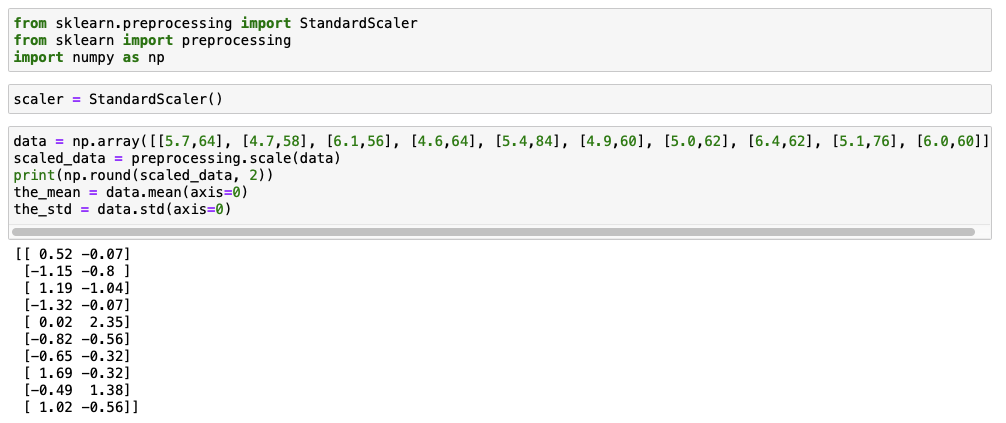
\includegraphics[scale=0.4]{img10} \\

b) \\
We scale the centroids. \\
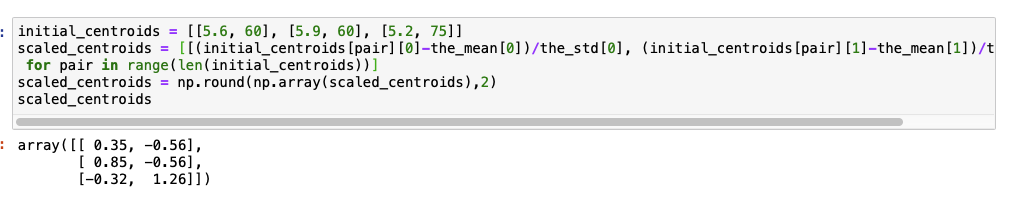
\includegraphics[scale=0.4]{img11} \\
\\
After one iteration we get. \\
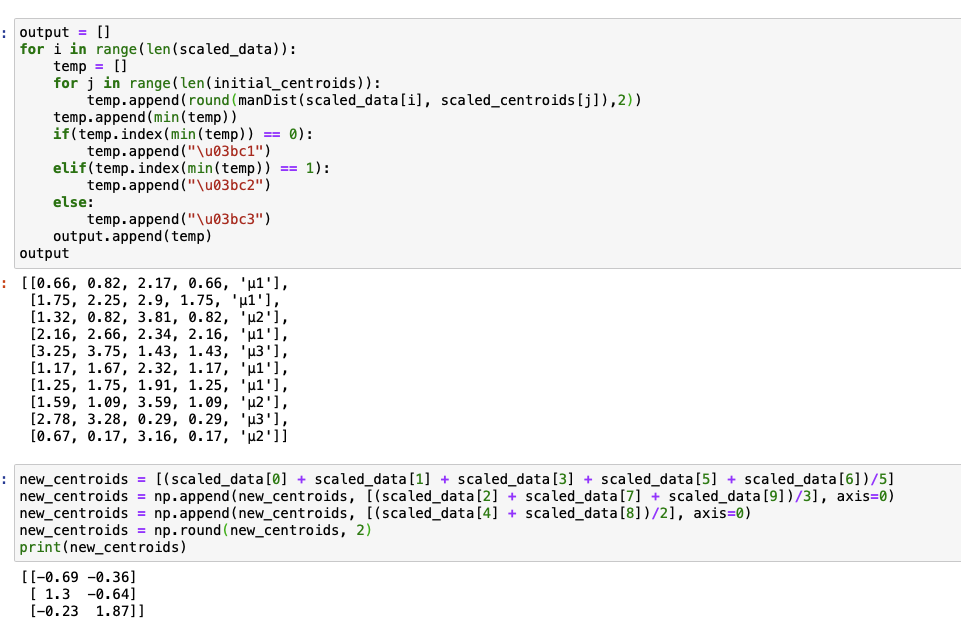
\includegraphics[scale=0.4]{img12} \\
\\ \\ 

After second iteration we get. \\
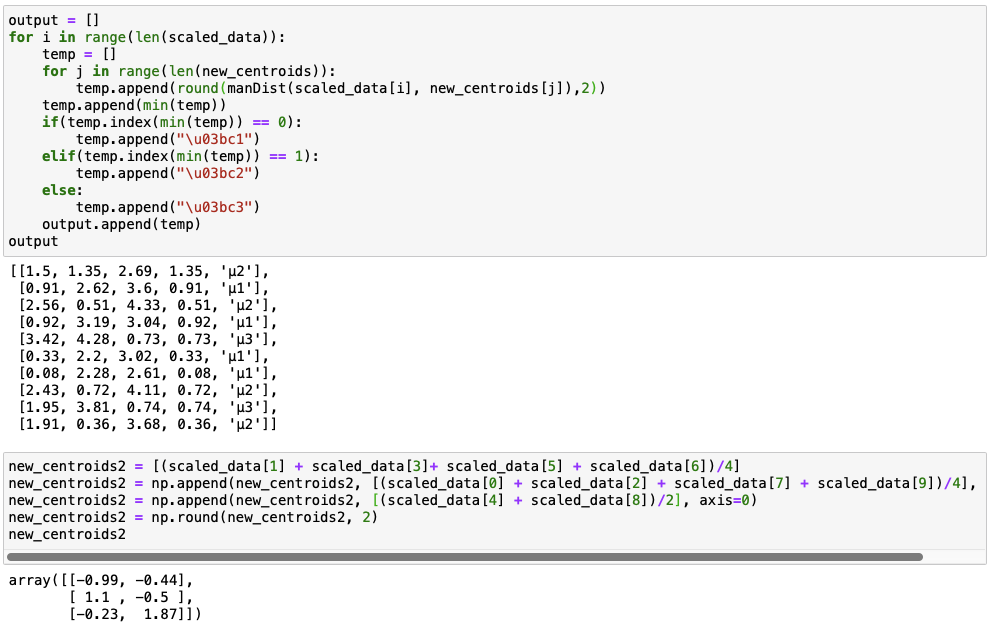
\includegraphics[scale=0.4]{img13} \\
\\
Center of second cluster [1.1, -0.5]. \\

c) \\
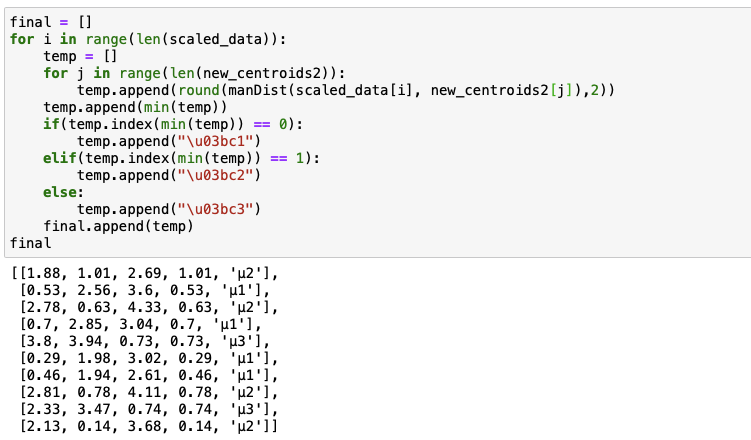
\includegraphics[scale=0.4]{img14} \\
The points did not change, therefore converged. The centroids are the same as before. \\
So center of third cluster is [-0.23, 1.87]. \\

d) \\
The points don't change after 3 iterations. Therefore, 3 iterations are required for cluster to converge. \\

2) \\
We pick the plot in each set where the points are assigned to the color of the cluster that is closest. The other plot in the set does not do that. \\
a) A2 \\
b) B2 \\
c) C2 \\
d) D1 \\
e) E2 \\
f) F2 \\
\\
3) \\ 
a) \\
complete linkage (maximum distance) \\
two farthest points are (4.6,2.9) and (6.7,3.1). \\
$d = ((6.7-4.6)^2 + (3.1-2.9)^2 )^{0.5} = 2.11$ \\
You also see it is the highest from the python code below where I calculated distance between all points. \\

b) \\
single linkage (minimum distance) \\
two closest points are (5,3) and (5.9,3.2). \\
$d = ((5.9-5)^2 + (3.2-3)^2)^{0.5} = 0.92$ \\
You also see it is the lowest rom the python code below where I calculated distance between all points. \\

c) \\
average link is 1.41 \\
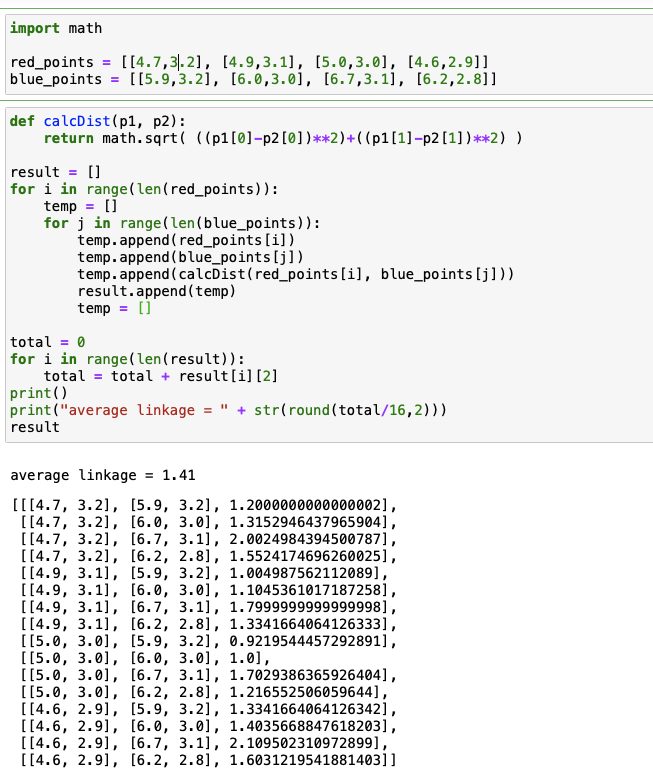
\includegraphics[scale=0.35]{img15} \\

d) \\
the average link is clearly the most robust to noise, but it takes longer to compute. \\ \\

4) (From Jupyter notebook) \\
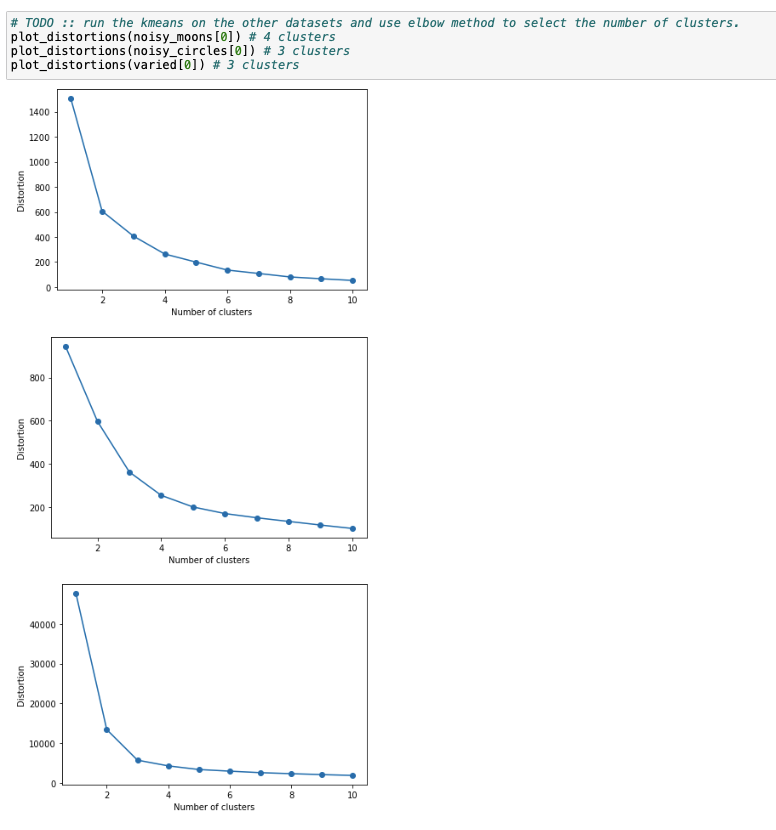
\includegraphics[scale=0.4]{img16} \\ \\ \\
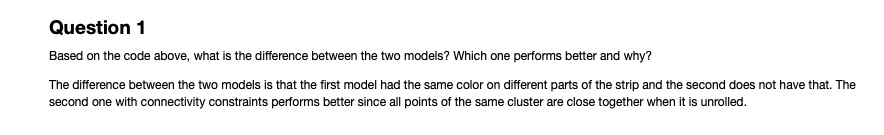
\includegraphics[scale=0.4]{img17} \\ \\ \\
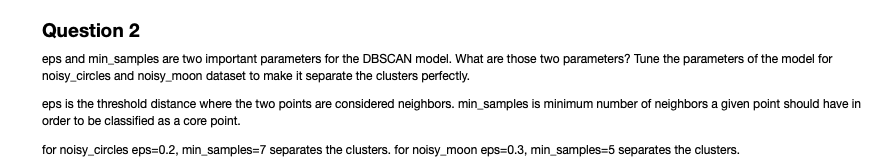
\includegraphics[scale=0.4]{img18} \\ \\ \\ \\ \\ \\ \\ \\ \\ \\ 


I used k means clustering on this data set I found. From the elbow method we see it's 3 or 4 clusters. I picked 3. \\
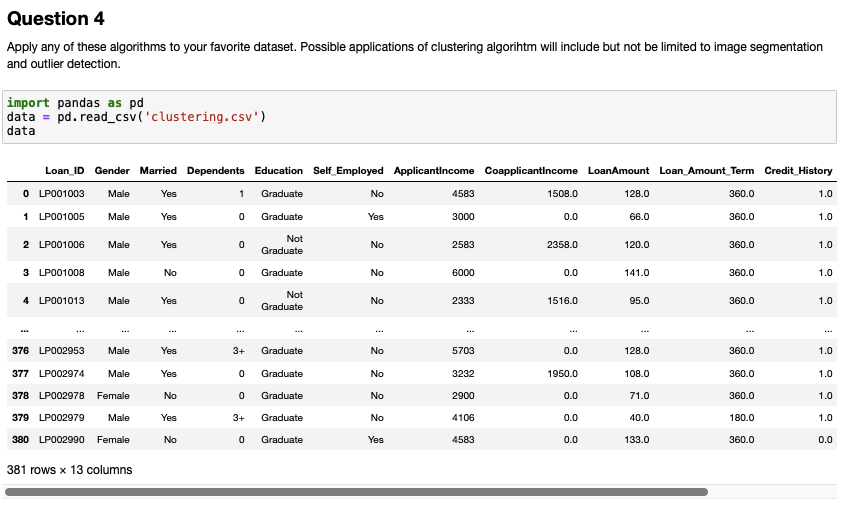
\includegraphics[scale=0.36]{img19} \\
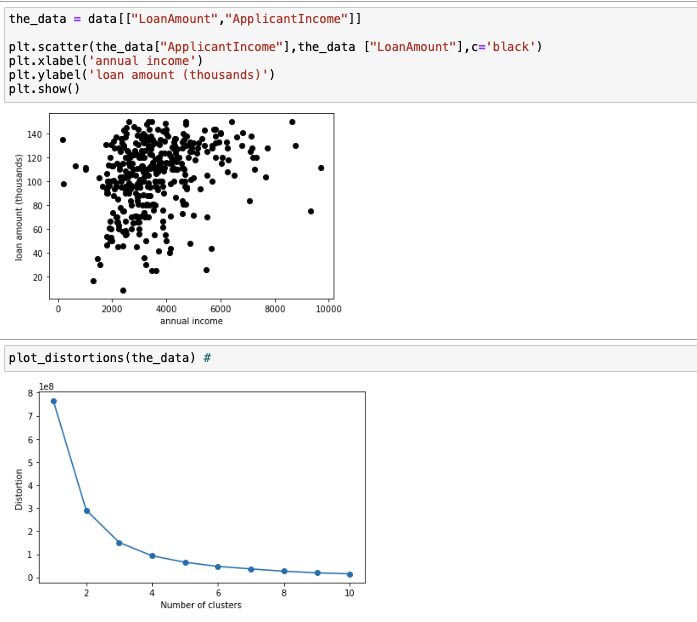
\includegraphics[scale=0.4]{img20} \\
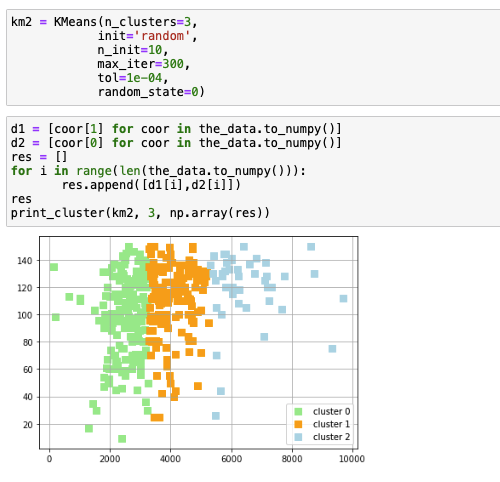
\includegraphics[scale=0.4]{img21} \\
\end{document}

